\begin{frame}{Getting started (1)}
  \begin{itemize}
    \item Keep in mind: This talk is only an introduction - there is more
    \item basic interaction with \git happens via the command line
    \begin{itemize}
      \item GUIs exist, but it is best to learn git from the command line
      \item Web-Frontends are widely used (we will talk about \github later)
    \end{itemize}
    \item git stores information for a single project in a \textit{git repository}
    \begin{itemize}
      \item commonly found on your hard disk in form of a folder
      \item \textit{clones} of the repository can be made in order to share it
    \end{itemize}

  \end{itemize}
\end{frame}

\begin{frame}{Getting started (2): Creating a repository}
  \begin{itemize}
    \item you can create a new repository in a folder by using \shellcmd{git init}
    \item alternatively you can clone an existing repository with \shellcmd{git clone repository-url}
    \item creates a \textit{working directory} where the current version is \textit{checked out}
    \item different versions are tracked with so-called \textit{commit}s
    \begin{itemize}
      \item has a title and some information when and by whom it was made
      \item stores a reference to the previous commit (version)
      \inote{not for the initial commit of course}
      \item stores the changes were made since that version
    \end{itemize}
  \end{itemize}
\end{frame}

\begin{frame}{Getting started (3): Working Directory, Staging Area \& History}
  \begin{columns}[onlytextwidth]
    \begin{column}{0.5\textwidth}
      \begin{itemize}
        \item commits are local to your clone - they are not automatically shared
        \item Making a commit
        \begin{itemize}
          \item first make changes in your working directory (also called the index)
          \item then add the files you want to commit to the staging area
          \item finally you commit the changes in the staging area
        \end{itemize}
      \end{itemize}
    \end{column}
    \begin{column}{0.5\textwidth}
      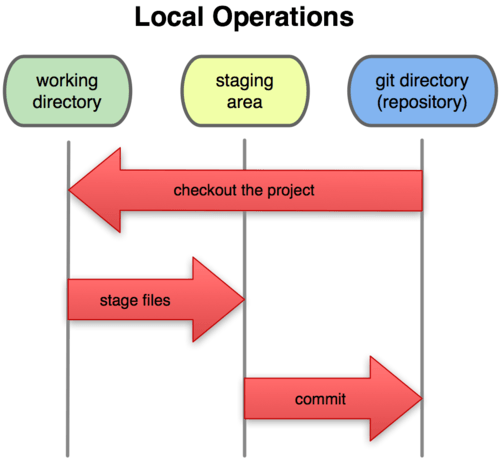
\includegraphics[width=0.95\textwidth]{imgs/git_local}
    \end{column}
  \end{columns}
\end{frame}

\begin{frame}{Getting started (4): Commands for creating commits}
  \begin{itemize}
    \item Commands for creating commits
    \begin{itemize}
      \item \shellcmd{git status} - to see what is changed and what is in the staging area
      \item \shellcmd{git add FILES} - to add files to the staging area
      \inote{use \shellcmd{git add -A .} to add everything}
      \item \shellcmd{git rm FILES} - to delete a file and add that change to the staging area
      \item \shellcmd{git commit -m MESSAGE} - to create a commit with the given message from the staging area
      \item \shellcmd{git checkout FILE} - to reset FILE to the last commit
    \end{itemize}
    \item Time for a short demo
  \end{itemize}
\end{frame}

\begin{frame}{Getting started (5): Sharing commits}
  \begin{itemize}
    \item Creating commits is great, but how to share them?
    \item git uses so called ``remotes''
    \inote{a remote is just a different clone of the same repository somewhere else}
    \item commits can be pushed to it -- using \shellcmd{git push}
    \item commits can be pulled from it -- using \shellcmd{git pull}
    \item internally it is a bit more complicated than that - we need to talk about branching first
  \end{itemize}
\end{frame}